% !Mode:: "TeX:UTF-8"
% !TEX program  = xelatex
\documentclass[AutoFakeBold,AutoFakeSlant,scheme=plain,degree=bachelor]{sustechthesis}
% 1. AutoFakeBold 与 AutoFakeSlant 为伪粗与伪斜,如果本机上有相应粗体与斜体字体,请使用 xeCJK 宏包进行设置,例如:
%   \setCJKmainfont[
%     UprightFont = * Light,
%     BoldFont = * Bold,
%     ItalicFont = Kaiti SC,
%     BoldItalicFont = Kaiti SC Bold,
%   ]{Songti SC}
%
% 2. scheme=chinese 为 ctexart 文类提供的中文排版方案,如果使用英文进行论文创作,请使用 scheme=plain 选项。
%
% 3. degree=bachelor 为 sustechthesis 文类提供的本科生毕业论文模板,其他可选项为 master 与 doctor,但是均未实现,如果您对此有兴趣,欢迎 PR。
%
% 4. sustechthesis.cls 文类主要参考自去年完成使命的 sustechthesis.tex,在这一年的时间,作者的 TeX 风格与常用宏包发生许多变化,因为之前的思想为仅提供必要的格式修改相关代码,所以转换为文类形式所进行的修改较少,而近期的风格与常用宏包均体现在以下的例子文件中。
%
% 5. 示例文件均放置于相应目录的 examples 文件夹下,构建自己论文时可暂时保留,用以检索接口与使用方法。

% !Mode:: "TeX:UTF-8"
% !TEX program  = xelatex

% 数学符号与环境
\usepackage{amsmath,amssymb}
  \newcommand{\dd}{\mathrm{d}}
  \newcommand{\RR}{\mathbb{R}}
% 参考文献
\usepackage[style=gb7714-2015]{biblatex}
  \addbibresource{ref.bib}
% 无意义文本
\usepackage{zhlipsum,lipsum}
% 列表环境设置
\usepackage{enumitem}
% 浮动题不越过 \section
\usepackage[section]{placeins}
% 超链接
\usepackage{hyperref}
% 图片,子图,浮动题设置
\usepackage{graphicx,subcaption,float}
% 抄录环境设置,更多有趣例子请命令行输入 `texdoc tcolorbox`
\usepackage{tcolorbox}
  \tcbuselibrary{xparse}
  \DeclareTotalTCBox{\verbbox}{ O{green} v !O{} }%
    {fontupper=\ttfamily,nobeforeafter,tcbox raise base,%
    arc=0pt,outer arc=0pt,top=0pt,bottom=0pt,left=0mm,%
    right=0mm,leftrule=0pt,rightrule=0pt,toprule=0.3mm,%
    bottomrule=0.3mm,boxsep=0.5mm,bottomrule=0.3mm,boxsep=0.5mm,%
    colback=#1!10!white,colframe=#1!50!black,#3}{#2}%
\tcbuselibrary{listings,breakable}
  \newtcbinputlisting{\Python}[2]{
    listing options={language=Python,numbers=left,numberstyle=\tiny,
      breaklines,commentstyle=\color{white!50!black}\textit},
    title=\texttt{#1},listing only,breakable,
    left=6mm,right=6mm,top=2mm,bottom=2mm,listing file={#2}}


% LaTeX logo
\usepackage{hologo}
 % 导言区
% !Mode:: "TeX:UTF-8"
% !TEX program  = xelatex
\设置信息{
%   键 = {{中文值}, {英文值}},
    分类号 = {{}, {}},
    编号 = {{}, {}},
    UDC = {{}, {}},
    密级 = {{}, {}},
    题目 = {{单细胞测序数据的}, {Dimensionality reduction of }},
    子标题 = {{降维方法研究}, {single-cell RNA-seq data}},
    姓名 = {{罗子翔}, {Zixiang Luo}},
    学号 = {{11612617}, {11612617}},
    系别 = {{生物系}, {Department of Biology}},
    专业 = {{生物信息学}, {Bioinformatics}},
    指导老师 = {{靳文菲, 张振}, {Wenfei Jin, Zhen Zhang}},
    时间 = {{2020年5月18日}, {May 18, 2020}},
}
 % 论文信息
\begin{document}

%\中文标题页\英文标题页
%\中文诚信承诺书\英文诚信承诺书
%\摘要标题
%% !Mode:: "TeX:UTF-8"
% !TEX program  = xelatex
\begin{中文摘要}{单细胞测序,降维,变分自编码器}
  单细胞测序技术使我们可以有效的发现组织中细胞间的异质性。降维对聚类和发育轨迹推断等后续分析有着关键的作用。在本研究中,我们提出了一种新的对单细胞测序数据降维的方法:针对零膨胀数据的变分自编码器(ZIVA)。它可以模拟单细胞测序数据中的数据丢失现象从而可以准确的可视化数据以及判断细胞类型。我们还系统的比较了我们的模型和其他六个常用的方法在六个数据集上的表现。ZIVA在多数情况下都有良好的可视化效果。
\end{中文摘要}

\begin{英文摘要}{scRNA-seq, Dimensionality reduction, Variational autoencoder}
  Single cell sequencing technology enable us to effectively identify cellular heterogeneity in healthy and disease tissues. Dimensionality reduction of high dimensional expression data is a critical step for the downstream analysis such as cell clustering and lineage inference. In this study, we proposed a new method for dimensionality reduction of scRNA-seq data: zero-inflated variational autoencoder (ZIVA). It can model the dropout events in scRNA-seq data and accurately identify cell sub-populations. We systematically compared our model with six other popular methods on six datasets. It shows that ZIVA perform well in most cases.
\end{英文摘要}
 % 论文摘要

%\目录\clearpage % 目录及换页

%% !Mode:: "TeX:UTF-8"
% !TEX program  = xelatex
\section{Introduction}

\subsection{single cell RNA sequencing}

In the past decades, bulk cell RNA sequencing was extensively used to study the gene expression features at the tissue level. However, it only reflects the averaged expression level of cells in a tissue. The rapid growth of single-cell RNA sequencing (scRNA-seq) technologies enables researchers to study the gene expression patterns at the single-cell level. It dramatically aids researchers in identifying molecular heterogeneity and better understand biological mechanisms \cite{shapiro2013single}. For example, the single-cell sequencing of cancer cells reveals the mutations on each sub-population of cells and helps construct the cancer development trajectory. 

\begin{figure}[htb!]
    \centering
    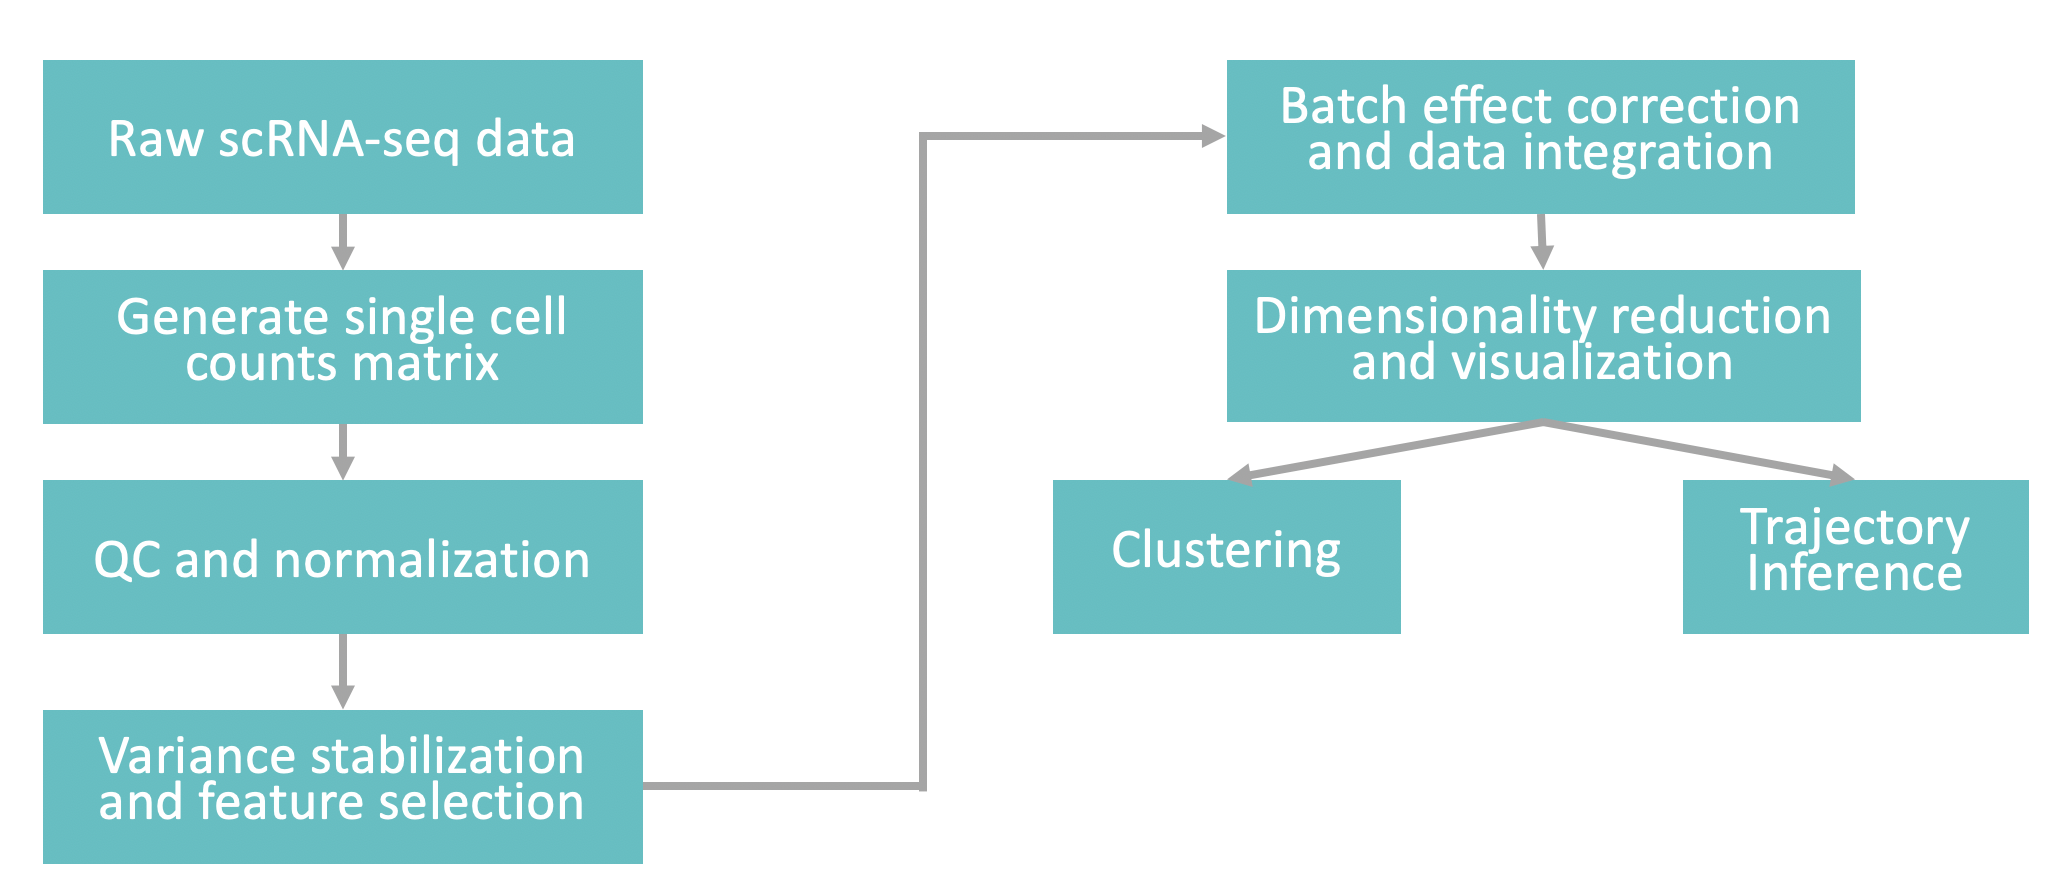
\includegraphics[width=1\textwidth]{figures/myfigures/scpip.png}
    \caption{The basic pipeline of scRNA-seq data analysis}
    \label{scpip}
\end{figure}

The primary pipeline of scRNA-seq analysis is shown in figure \ref{scpip}. Firstly, the raw sequencing FASTQ files should be processed to a count matrix. In this process, each read's sequence is aligned to a reference genome to find out the gene that read belongs to. In this way, the count matrix can be generated \cite{petukhov2017accurate}. The value at the $i^{th}$ row and $j^{th}$ column is the expression value of gene$j$ at the cell $i$.

Then, identify the corresponding cell by the cell barcode in the sequence. After getting a count matrix, quality control should be performed to remove technical biases and noises \cite{van2017single}. It usually involves removing dead cells by filtering out the cells with low reads or high mitochondrial reads and removing doublets. Also, a proper normalization, such as total count normalization or Sctransform normalization, helps identify additional cell heterogeneity \cite{vallejos2017normalizing}. Besides from normalization, variance stabilization and batch effect removing also make the downstream analysis easier.

The downstream analysis mainly consists of dimensionality reduction, clustering, trajectory inference, and cell-type annotation. Dimensionality reduction can represent the high dimensional scRNA-seq data in a low-dimensional space and thus benefit clustering and trajectory inference processes. scRNA-seq datasets usually contain some distinct cell types or the cells in continuous changes. For the cells that can be divided into several discrete types, cluster clustering can be performed to assign each cell to a cluster with the same type of cells. The most common clustering method for single-cell sequencing data is the Louvain algorithm \cite{traag2019louvain}. It uses a community detection algorithm to add data points to communities iteratively and thus clusters the cells. For those continuous cell types, trajectory inference is usually performed to resolve the cell development lineage. Monocle2 uses reverse graph embedding to learn the graph structure of the data in a high dimensional space and a low dimensional space at the same time \cite{qiu2017reversed}. Clustering and trajectory inference is usually performed based on the result of dimensionality reduction. Finally, cell type annotation is usually performed by identifying the genes that are uniquely expressing in a cluster and match the gene to the database of empirical cell type markers \cite{abdelaal2019comparison}. 

\subsection{Dimensionality reduction}

The single-cell sequencing data usually have more than two thousand dimensions, which makes it challenging to be analyzed directly. Thus, finding a meaningful low dimensional representation to represent those cell states is a necessary step in scRNA-seq data analyzing. Those genes are highly regulated and co-expressed. There is much redundant information in the dataset because only a limited number of cell states are in a group of cells. It is assumed that those data form a low dimensional manifold in a high dimensional space. The dimensionality reduction process can extract the crucial information in the original high dimensional data and represent it as a low-dimensional structure \ref{dr1}.  It plays a vital role in data visualization and data preprocessing, which allows efficient downstream analysis such as trajectory inference \cite{Saelens2019}, cell clustering \cite{weber2016comparison}, and cell sub-population identification \cite{Hwang2018}. 

\begin{figure}[htb!]
    \centering
    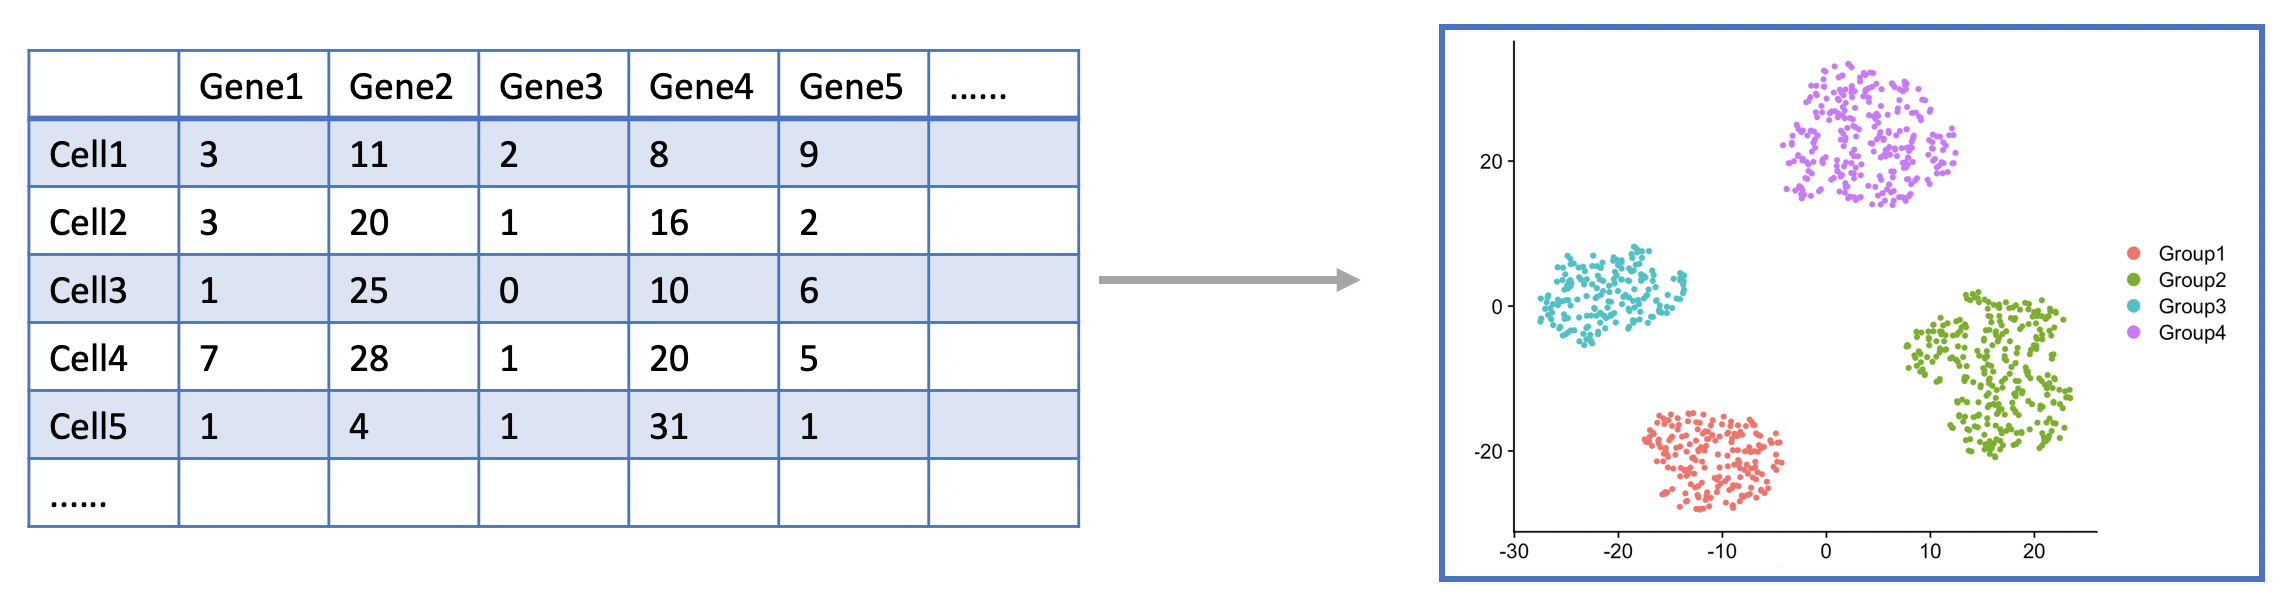
\includegraphics[width=1\textwidth]{figures/myfigures/dr1.png}
    \caption{Dimensionality reduction of sequencing data}
    \label{dr1}
\end{figure}

For example, Seurat uses PCA \cite{Abdi2010} to reduce dimensionality before clustering \cite{Satija2015}. Destiny \cite{angerer2016destiny} uses diffusion map before clustering. Monocle \cite{Qiu2017} performs uniform manifold approximation and projection (UMAP) \cite{McInnes2018} or independent component analysis (ICA) \cite{hyvarinen2000independent} before inferencing cell trajectories. 

The most classic and most common dimensionality reduction method is principal component analysis (PCA). PCA performs dimensionality reduction by iteratively finding the direction that can explain most variance and project points to that direction as a component. The first two principal components are usually chosen as coordinates to visualize data points. However, scRNA-seq datasets are usually non-linear because the relationship between genes is often non-linear. Thus, the linear dimensionality reduction methods such as PCA and MDS \cite{Kruskal1964} have some limitations. Non-linear methods usually have better performance for visualization of scRNA-seq data.

The most popular non-linear dimensionality reduction method is t-distributed stochastic neighbor embedding (tSNE). It calculates the similarity between data points in high dimensional space and low dimensional space and tries to keep the similarity distribution in two spaces as close as possible. By recovering the similarity relationships between cells, tSNE can considerably preserve local structures and can form delicate clusters in visualization.  However, tSNE cannot preserve global structures well. The size and spatial relationship of clusters are often random \cite{wattenberg2016how}. Another non-linear dimensionality reduction method UMAP is developed in recent years. It has a similar visualization performance with tSNE \cite{kobak2019umap} but have lower running time and more reproducibility than tSNE \cite{becht2019dimensionality}.

\subsection{Dropout events}

However, the single-cell sequencing data have more noise than bulk cell data because of the low RNA capture efficiency and incomplete reverse transcription in single-cell sequencing \cite{Peng2019}. Some studies estimate that only 10\%-15\% of RNA in a cell can be captured and transcribed \cite{zheng2017massively}. Thus, single-cell sequencing data usually have excessive dropouts, which means many data points that should have more significant value are presented as zero or a value lower than the exact expression, which is shown in figure \ref{dropout}.

\begin{figure}[htb!]
    \centering
    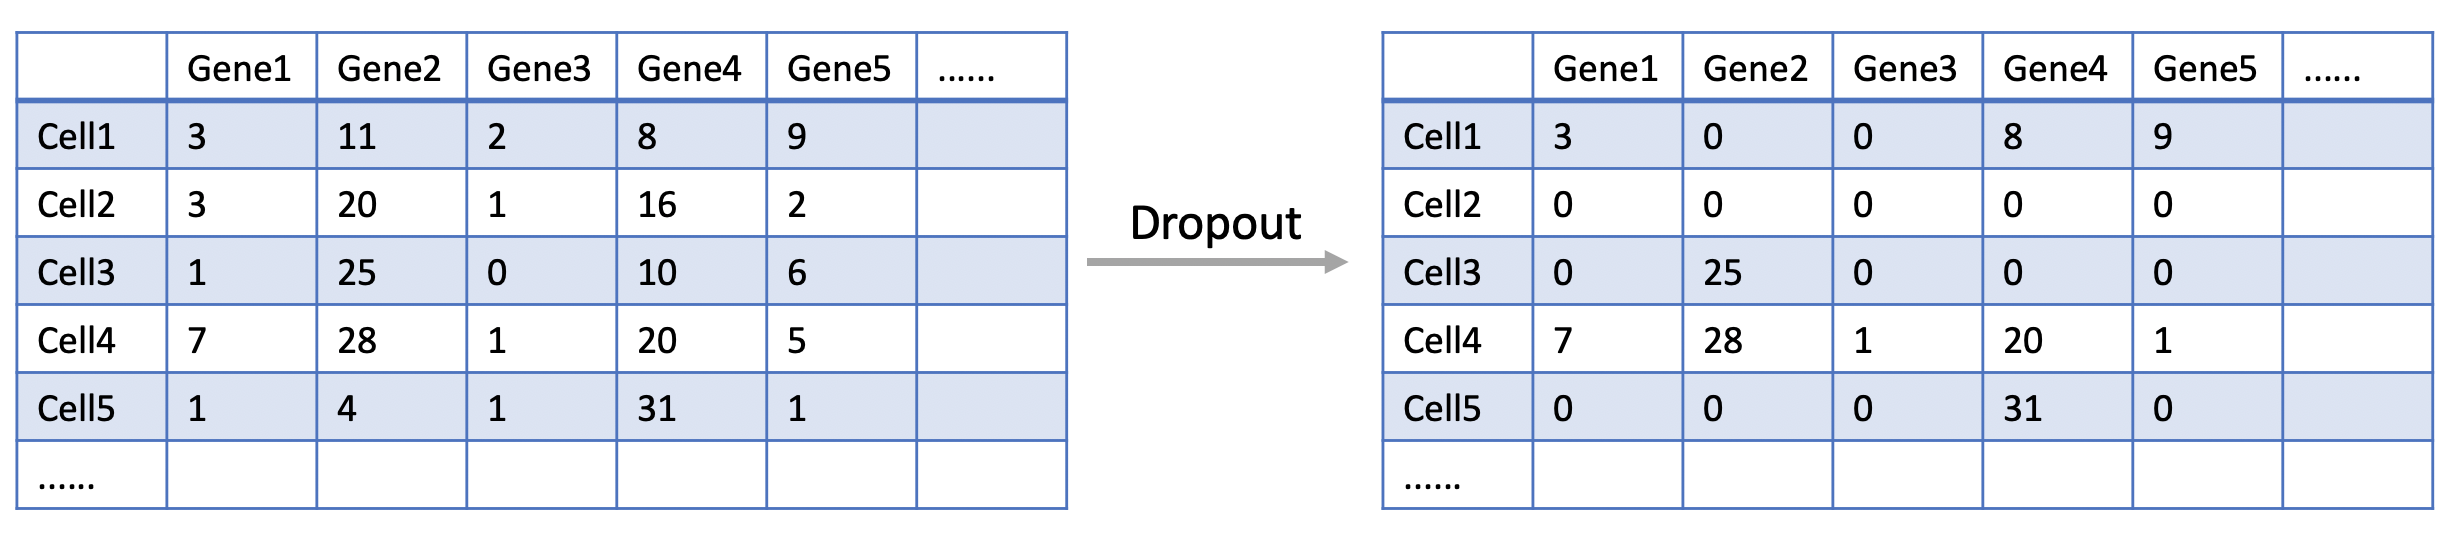
\includegraphics[width=1\textwidth]{figures/myfigures/dropout.png}
    \caption{The process of dropout to scRNA-seq data}
    \label{dropout}
\end{figure}

Some traditional methods cannot effectively extract the features which cause dimensionality reduction more difficult because of these noises. The visualization performance also decreases. Sometimes, the data points get mixed, sometimes it can be separated but is very dispersed, such as in figure \ref{dr2}.

\begin{figure}[htb!]
    \centering
    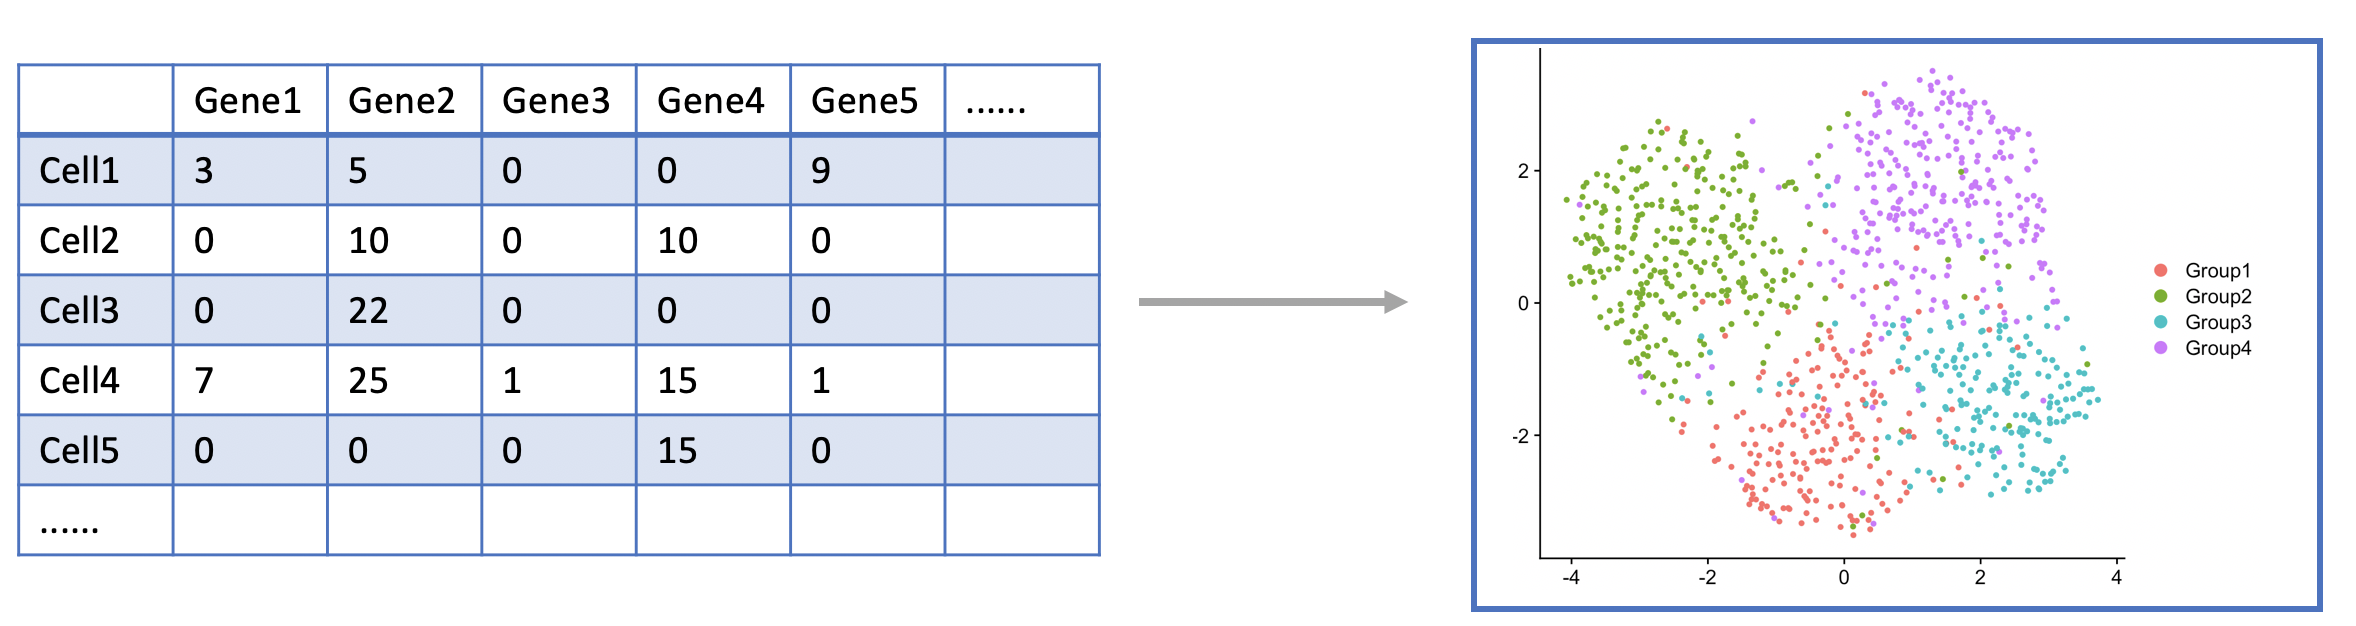
\includegraphics[width=1\textwidth]{figures/myfigures/dr2.png}
    \caption{Dimensionality reduction of scRNA-seq data with dropouts}
    \label{dr2}
\end{figure}

Many imputation methods are developed recently to impute those missing points. One kind of strategy, including MAGIC \cite{van2017magic}, RESCUE \cite{Tracy2019}, scImpute \cite{Li2018} and DrImpute \cite{gong2018drimpute}, borrows information of the same gene from other similar cells that don't have dropouts on that gene. Similar cells are chosen based on the genes that are unlikely to be affected by dropouts.

Some strategy performs imputation and clustering or dimensionality reduction at the same time \cite{lin2017cidr}. For example, ZIFA \cite{Pierson2015} performs dimensionality reduction while imputing the missing values at the same time. It probabilistically models the conditional dropout events and uses the EM algorithm \cite{mclachlan2007algorithm} to refer the model parameters and latent variables iteratively. 

With the fast development of deep learning in recent years, some approaches make use of deep learning technologies. scScope \cite{Deng2019} uses a recurrent neuron network to impute the missing values. scGAIN \cite{gunady2019scgain} uses a generative adversarial network (GAN) to learn the distribution of the scRNA-seq data and impute the missing values. GraphSCI \cite{rao2020imputing} uses graph convolution neuron network and makes use of gene-gene interaction to impute scRNA-seq data. Moreover, some methods build the model based on autoencoder or variational autoencoder. In this way, the bottleneck layer can be used for dimensionality reduction. For example, VASC \cite{Wang2018} adds the dropout model in ZIFA to a VAE model to enable it to model the dropout events. DCA \cite{Eraslan2019a} uses autoencoder to impute the missing values by assuming the zero-inflated negative binomial model \cite{Hafemeister2019}. 

\subsection{ZIVA model}
In this study, I compared the performance of several popular dimensionality reduction methods on visualization, clustering, and trajectory inference of scRNA-seq data. Also, based on the structure of VAE \cite{Kingma2014}, I improved the model of VASC \cite{Wang2018} and proposed a new method, zero-inflated variational autoencoder (ZIVA), to analyze and visualize the single-cell RNA sequencing data. It uses the Gumbel softmax and double-exponential function to model the dropout events. The comparison results show that ZIVA has excellent performance on cell clustering and cell trajectory inference tasks.
%% !Mode:: "TeX:UTF-8"
% !TEX program  = xelatex
\section{Methods}
\subsection{Variational autoencoder}
I used a modified variational autoencoder \cite{Kingma2014} to reduce the dimensionality of the single cell RNA-seq data. The autoencoder is composed of an encoder network and a decoder network \cite{wang2016auto}. The encoder network aims to model the distribution of the data points $P(x)$ in a high dimensional space $X$ and represents them by low dimensional latent variables $z$. Then, the decoder network maps the low-dimensionality variables $z$ back to the original high dimensional space $X$. To ensure that the generated latent representation $z$ can extract the intrinsic features of the data points, autoencoder tries to keep the reconstructed outputs and the original inputs as close as possible. \\
However, the autoencoder only minimize the reconstruction error between the input data and the decoded data. The network is likely to be overfitted, which may cause bad effects to the visualization of data points. So, the variational autoencoder model adds regularizations to the original autoencoder in order to avoid overfitting and get more meaningful visualization results. Instead of encoding the data as a point in the latent space, VAE encodes the data as a distribution in the latent space. A point is sampled from that distribution each time to feed into the decoder network. \\
Theoretically, the optimal distribution of $z$ follows the posterior probability $P(z|x)$, which is usually intractable. Therefore, VAE hopes to use a variational probability $Q(z|x)$ to approximate that posterior probability \cite{doersch2016tutorial}. It minimizes the $KL$-divergence between them:
\begin{equation}
\boldsymbol{D}[\boldsymbol{Q}(\boldsymbol{z} | \boldsymbol{X}) \| \boldsymbol{P}(\boldsymbol{z} | \boldsymbol{X})]=\mathbf{E}_{z \sim Q}[\log \boldsymbol{Q}(\boldsymbol{z} | \boldsymbol{X})-\log \boldsymbol{P}(\boldsymbol{z} | \boldsymbol{X})]
\end{equation}
Using Bayes rule and reordering the formula, it is equivalent to maximizing the following equation:
\begin{equation}
\mathbf{E}_{z \sim Q}[\log \boldsymbol{P}(\boldsymbol{X} | \boldsymbol{z})]-\boldsymbol{D}[\boldsymbol{Q}(\boldsymbol{z} | \boldsymbol{X}) \| \boldsymbol{P}(\boldsymbol{z})]
\end{equation}
Where $E$ means the expectation of $z$ which is sampled from distribution $Q$. $P(X|z)$ can be modeled by a decoder and $Q(z|X)$ can be modeled by an encoder. The first term can be viewed as the reconstruction loss. The second term minimizes the $KL$-divergence between the latent variable distribution and the normal distribution. It forces the latent variables follow the standard Gaussian distribution.
\subsection{Model structure}
The whole structure of ZIVA is shown in Figure 1. The details of model design and optimization algorithms are described as following. 
\begin{figure}
    \centering
    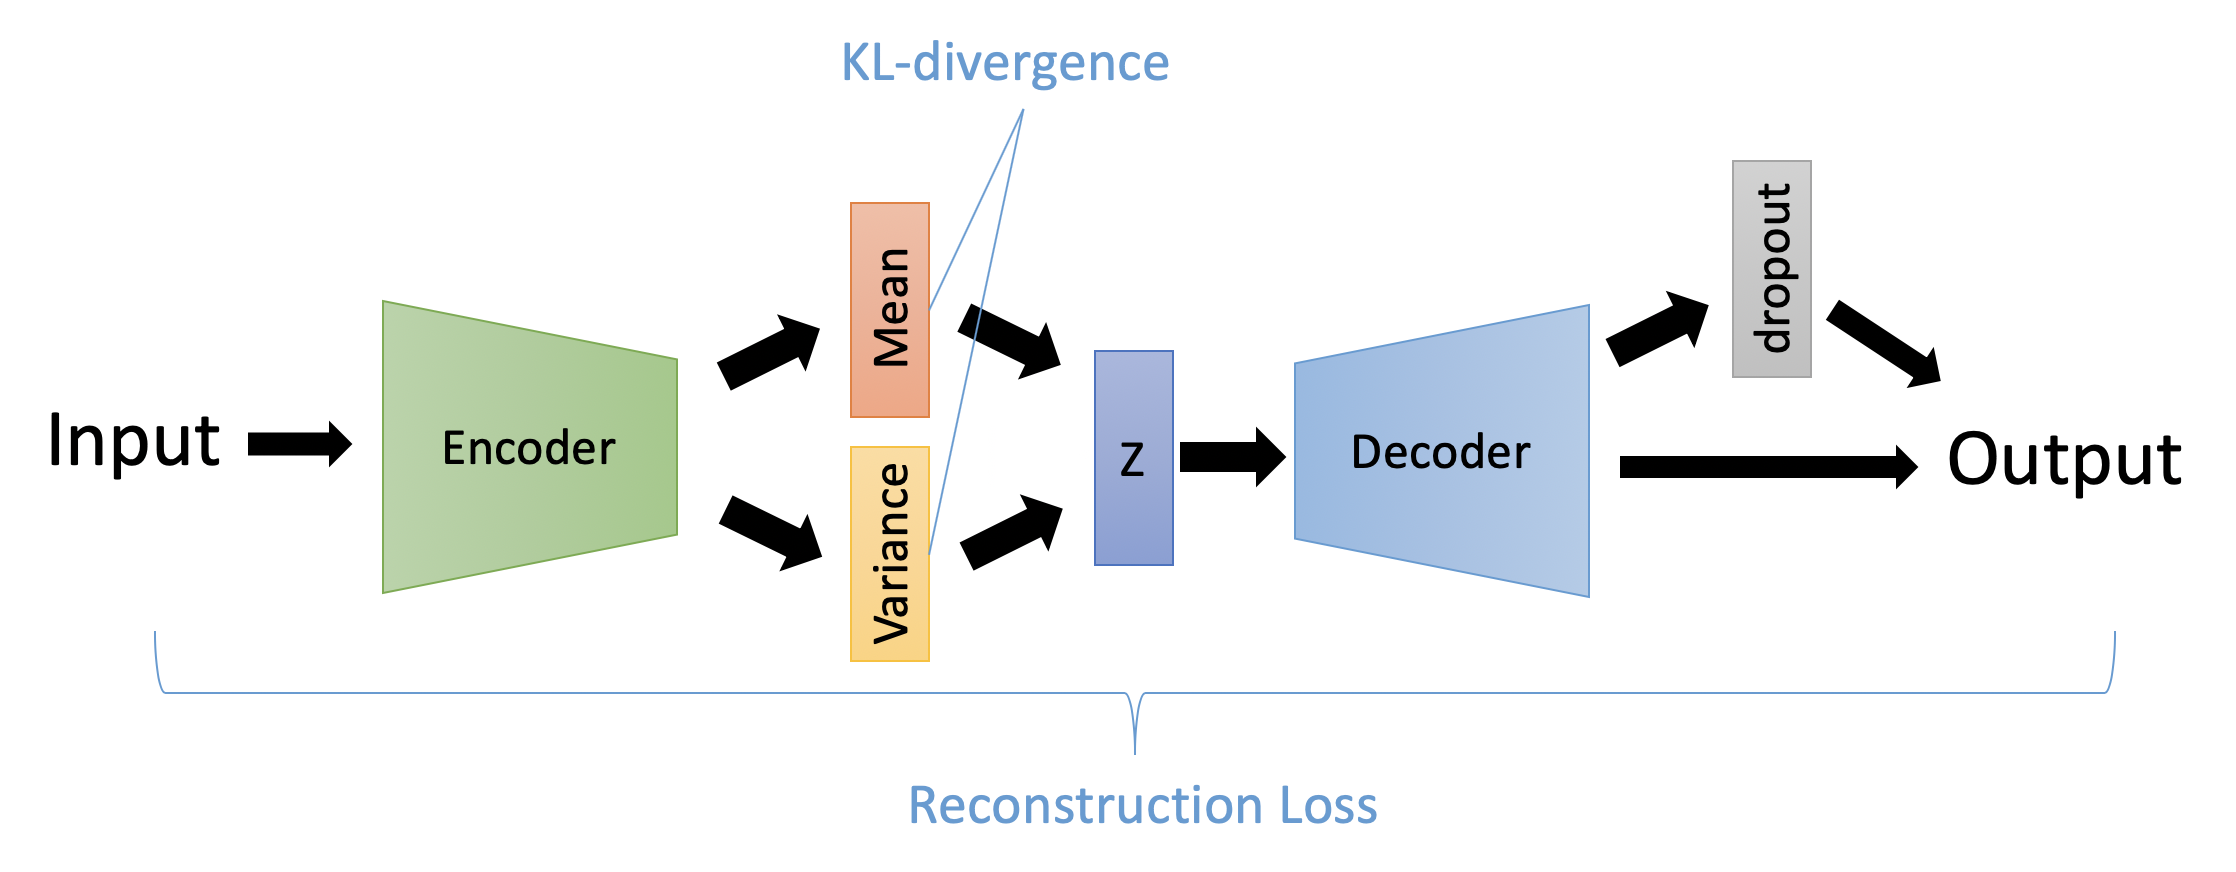
\includegraphics[width=1\textwidth]{figures/myfigures/ZIVA.png}
    \caption{The whole structure of ZIVA}\label{F:test-a}
    ZIVA mainly contain three parts: an encoder network, a decoder network and a zero-inflation model. 
\end{figure}

\vspace{0.5cm}
\noindent\emph{Input layer} \\ The ZIVA model uses the expression value matrix from single cell RNA sequencing data as inputs. Then, the data were performed log transformation to improve robustness of the model.  Also, the expression of genes in a cell were re-scaled to 0-1 by dividing the maximum gene expression value in the same cell. 

\vspace{0.5cm}
\noindent\emph{Dropout layer} \\ A dropout layer \cite{baldi2013understanding} is followed by the input layer. This layer sets some value to zero to get better performance of learning \cite{vincent2008extracting}. It can be viewed as some artificial dropouts which can force the model to learn to aid the bad effect of dropout noises. 

\vspace{0.5cm}
\noindent\emph{Encoder network} \\
The encoder network aims to represent the data points in a low-dimensionality latent space. It is composed of three fully connected layers with 512, 128 and 32 hidden units respectively. The first layer doesn’t have activation function. It can be viewed as a PCA transformation which makes the network more robust. Batch normalization layers was added before activation functions to increase the robustness. The l1-regularization was added to this layer which performs the feature selection function by forcing the sparsity of this layer. The last two layer were followed by ReLU activation function that perform non-linear transformation \cite{krizhevsky2012imagenet}.

\vspace{0.5cm}
\noindent\emph{Latent variable layer} \\
Followed by the last layer of the encoder network with 32 dimensions, the latent layer outputs the mean and variance of the latent variable with the latent dimension. Then, z was sampled from that mean and variance. A reparameterization trick was used to ensure the network is differentiable and can be trained by backward propagation.

\vspace{0.5cm}
\noindent\emph{Decoder network} \\
The decoder network aims to recover the original data points from latent variables z. It contains three fully connected layers with increasing dimensions 32, 128 and 512 respectively and an output layer. All of four layers use ReLU activation function. 

\vspace{0.5cm}
\noindent\emph{ZI layer} \\
Unlike the traditional VAE model, an additional zero-inflation (ZI) layer was added after the decoder network. The ZI layer models the dropout events in scRNA-seq data. It artificially set some points to zero according to the expression value of that gene. Specifically, it counts the probability of each data point to be dropout and sample a one-hot mask from that probability. Then, set some of points to zero by multiplying the mask and the output of the decoder network to get the final output. In this way, it forces the decoder to output the recovered data which is close to the true value of the gene expression. Two zero-inflation model were tested. The first is the model in ZIFA \cite{Pierson2015} which model the dropout rate based on a double exponential function: 
\begin{equation}
    P_{\text {dropout}}=\exp \left(-\lambda \mu^{2}\right)
\end{equation}
where $\mu$ is the log of expression level of a gene and $\lambda$ is a fitted parameter. The genes that have higher expression value have lower dropout probability. \\
The second model is proposed in \cite{andrews2017modelling} which is based on the Michaelis-Menten function:
\begin{equation}
    P_{\text {dropout}}=1-\frac{S}{\lambda+S}
\end{equation}
Where $S$ is the expression level of a gene and $\lambda$ is a fitted parameter. 
Both models fit the experimental data well. According to the experiment, the double exponential model fits the log-transformed data better. The Michaelis-Menten model fits the original counts data better. 
The parameter was fitted between the dropout rate (the percentage of zeros in the counts of a gene) and mean expression of that gene.
However, the backward propagation cannot deal with sampling process because it is non-differentiable. Here, we used the gumbel-softmax \cite{jang2016categorical} to approximate the sampling process. Suppose p is the dropout probability, q = 1-p. The sample s can be obtained by gumbel-softmax trick:
\begin{equation}
    \boldsymbol{s}=\frac{\boldsymbol{e} \boldsymbol{x} \boldsymbol{p}\left(\frac{\log \boldsymbol{p}+\boldsymbol{g}_{0}}{\tau}\right)}{\boldsymbol{e x p}\left(\frac{\log \boldsymbol{p}+\boldsymbol{g}_{0}}{\tau}\right)+\boldsymbol{e} \boldsymbol{x} \boldsymbol{p}\left(\frac{\log \boldsymbol{q}+\boldsymbol{g}_{1}}{\tau}\right)}
\end{equation}
where $g0$ and $g1$ were Gumbel noises that are sampled from a Gumbel distribution. They can be obtained by first sampling $u$ from a uniform distribution $\boldsymbol{u} \sim \text {Uniform}(0,1)$ and then compute $g$ from $\boldsymbol{g}=-\log (-\log \boldsymbol{u})$. Temperature $\tau$ can be set between 0 and 1. As it is closer to 0, the generated sample $s$ will be closer to the samples from the Bernoulli distribution. When $tau$ is too small, the gradient also becomes small and the optimization of the whole network can be hard. Therefore, setting $tau$ to 0.5 is a proper choice. For datasets with large sample sizes, we can use annealing strategy to gradually decrease $tau$.

\vspace{0.5cm}
\noindent\emph{Loss function} \\
\begin{equation}
    \operatorname{Loss}(X, Y)=\text {MSE}(\boldsymbol{X}, \boldsymbol{Y}) + 
    KL[\boldsymbol{Q}(\boldsymbol{z} | \boldsymbol{X}) \| \boldsymbol{P}(\boldsymbol{z})] + \lambda\|\mathbf{\widetilde{\boldsymbol{Y}}}\|_{*}
\end{equation}
As shown in the equation3, the first part of the loss function is reconstruction error between input and output data. The second part is the $KL$-divergence between the distribution of $z$ and the standard normal distribution. Also, we added the third part to the original VAE loss function which is the rank of the output matrix from decoder $\widetilde{\boldsymbol{Y}}$ . Nuclear norm was used to approximate the rank. In this way, the rank of the recovered matrix should be as small as possible because there are only limited number of distinct cell types. 

\vspace{0.5cm}
\noindent\emph{Optimization} \\
We used mini-batch gradient descent to optimize the whole structure. We chose the Adam optimizer with learning rate 0.0001. The source code can be found at \url{https://github.com/Zixiangluo/ZIVA}.


% !Mode:: "TeX:UTF-8"
% !TEX program  = xelatex
\section{Performance assessment}
\subsection{Visualization}
To evaluate the performance of ZIVA, we tested the visualization result of ZIVA and six other popular methods including PCA [], tSNE [], UMAP [], ZIFA [], VASC [] and ivis [] on 6 datasets with different number of cells and different sequencing protocols (Table \ref{datasets}). The visualization result is shown in Figure \ref{vis}.
\begin{figure}[htb!]
    \centering
    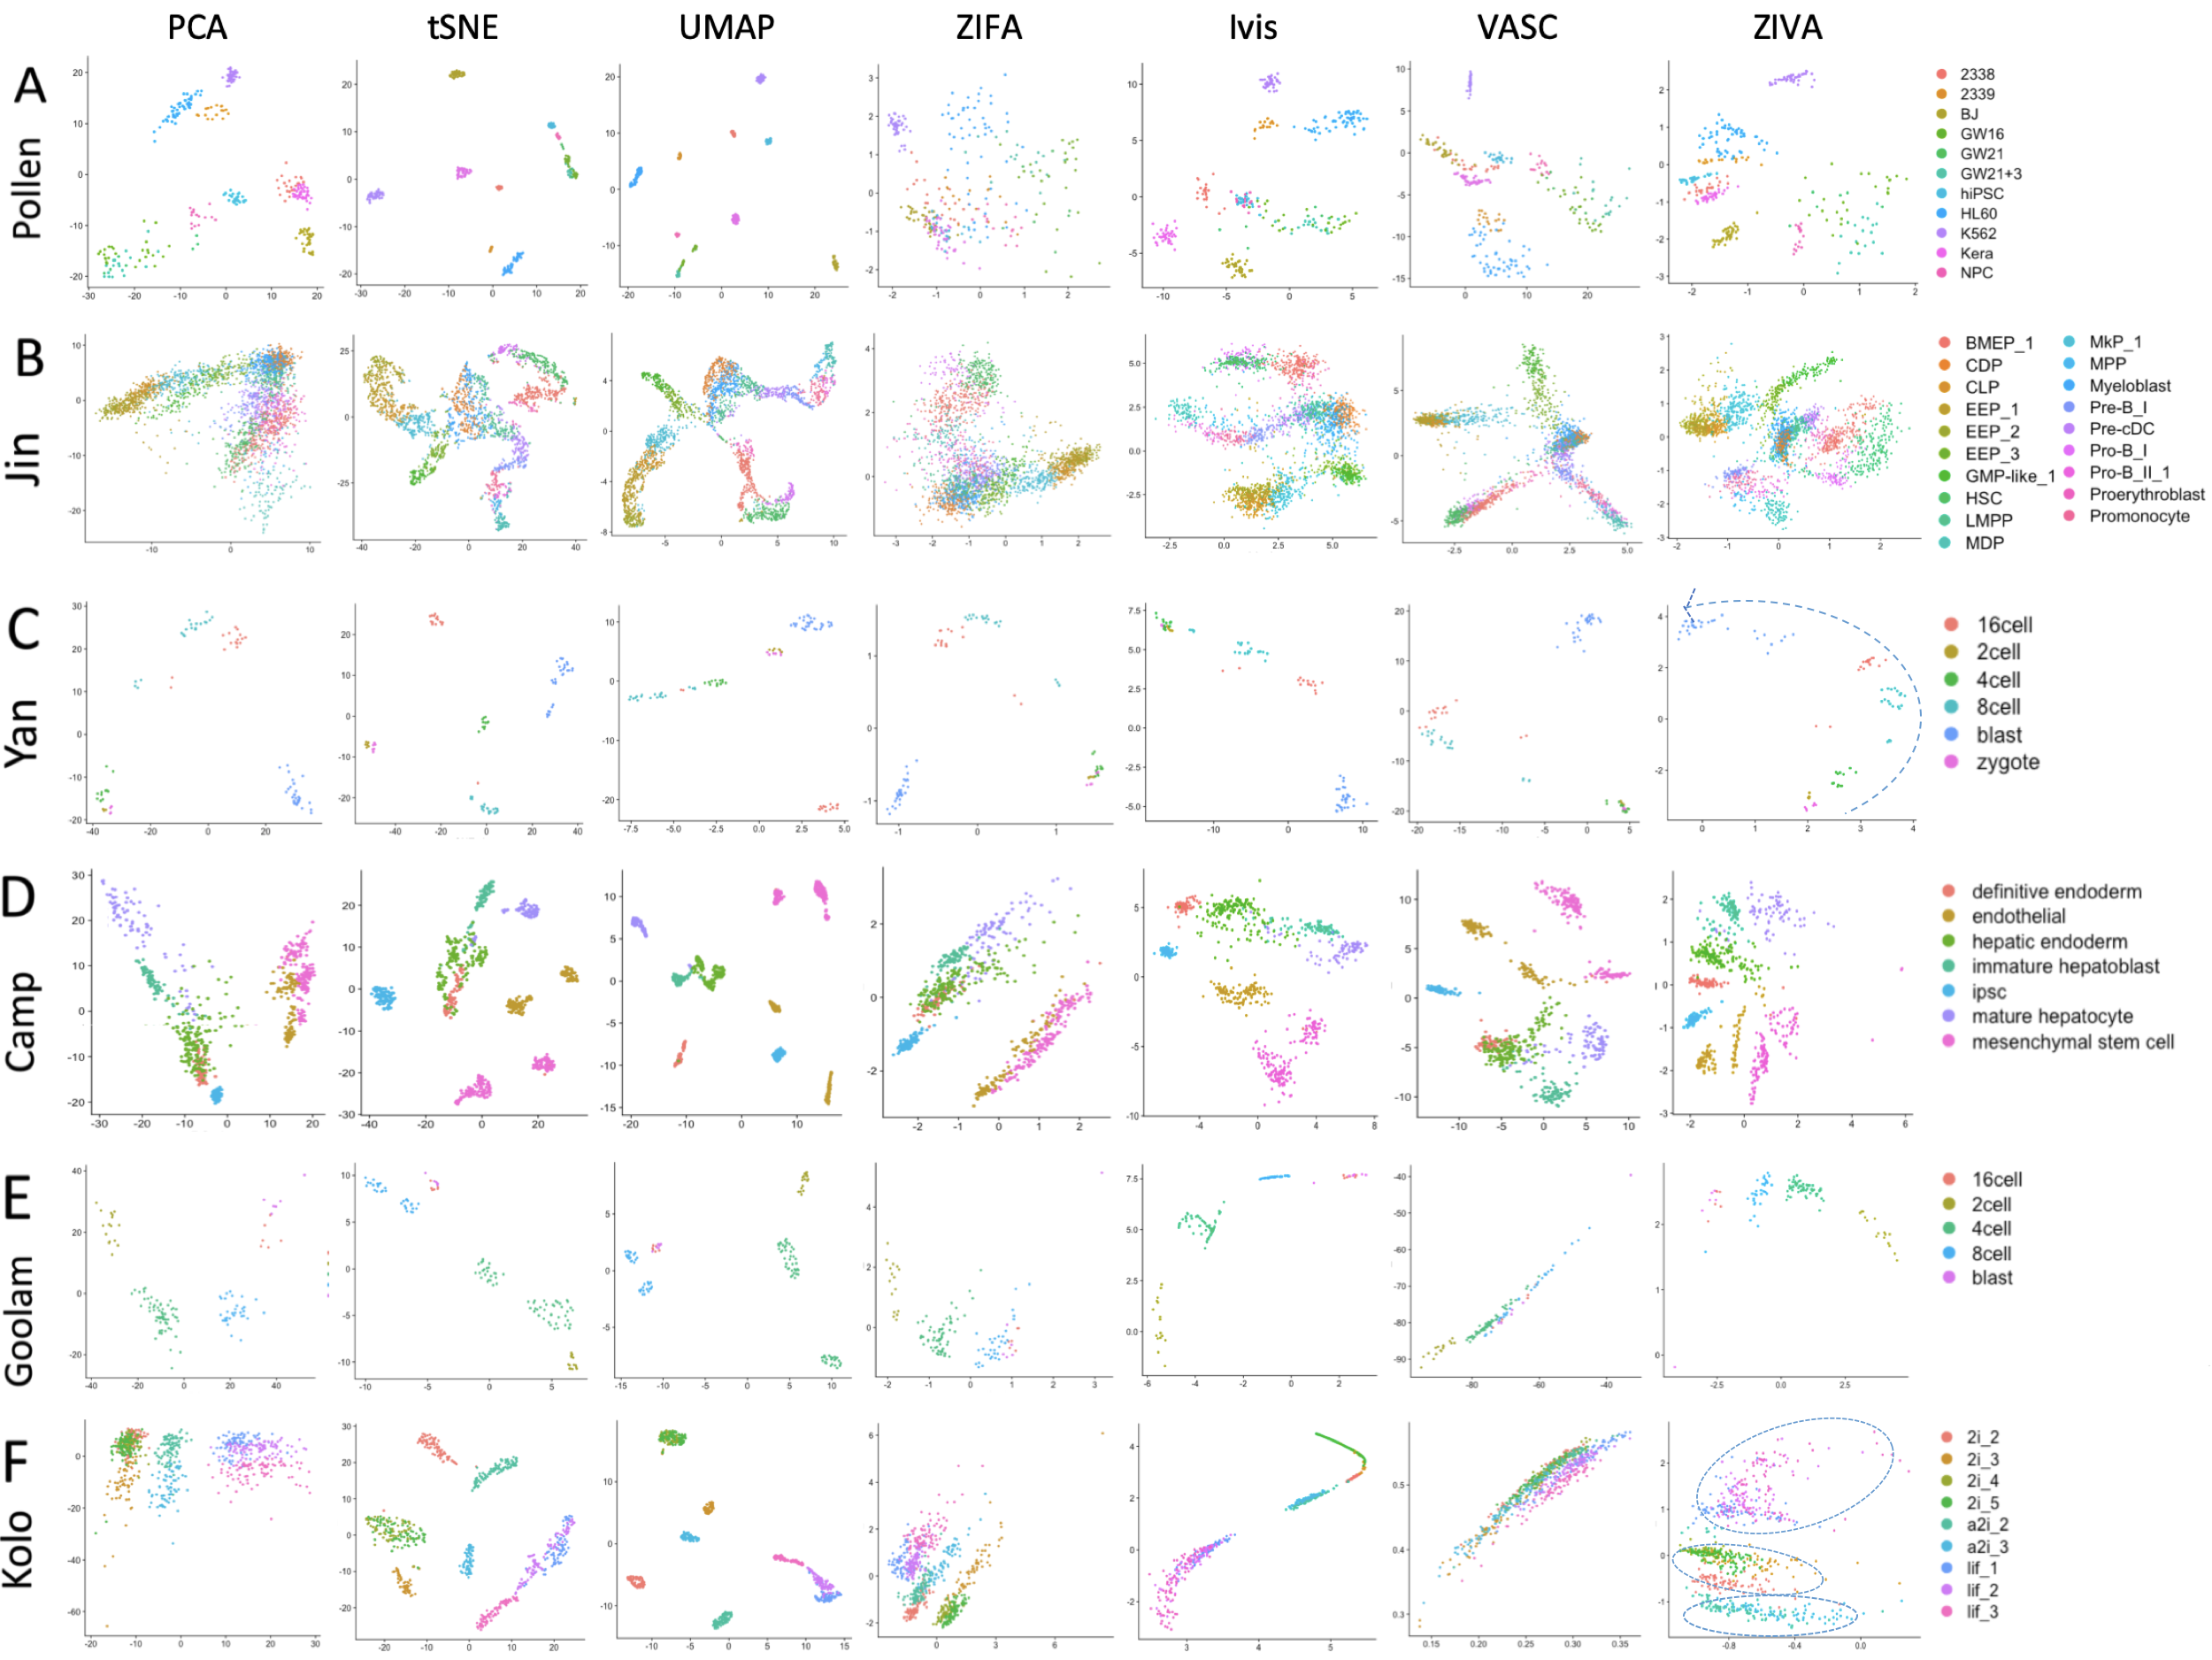
\includegraphics[width=1\textwidth]{figures/myfigures/visualizations.png}
    \caption{Visualization of scRNA-seq datasets}
    \label{vis}
\end{figure}
The results show that ZIVA has great performance all of six datasets. The clusters in the datasets can be well identified and cell lineages are also well recovered. For example, the Pollen dataset (Figure2.A) contains eleven different types of cells including blood, dermal, neural and pluripotent cells. ZIVA and most other methods except ZIFA can clearly separate them to different clusters. \\
The Yan dataset (Figure2.C) contains several types of embryonic cells from zygote to blast. VASC not only separate different cell types perfectly, but also greatly reconstructed the developmental stages of the cells. We can tell the developmental lineage (zygote, 2cell, 4cell, 8cell, 16cell, blast) from the visualization by ZIVA. PCA, Ivis, VASC and ZIFA also generated the lineage structure, but not as clear as in ZIVA. However, tSNE and UMAP that focus on local structure didn’t successfully recover the developmental relationships. It shows that ZIVA has superior performance on modelling embryo development progression than ZIFA, tSNE and UMAP. \\
The Kolodziejczyk dataset contains the embryonic cells grown from three different conditions: serum, 2i and alternate 2i (a2i). Under each condition, there are different batches of cells. It can be seen that ZIVA, Ivis and ZIFA well separated different culture conditions and several batches. PCA can also separate the conditions but batches are slightly mixed. VASC generated a mussy result. tSNE and UMAP formed beautiful clusters but failed to distinguish three conditions.
\subsection{Clustering performance}
Next, to quantitatively measure the performance of different methods, we evaluate the result of visualization by applying clustering to the dimensionality reduced 2D data. We used K-means to cluster cells and set k to the number of known cell types. Then, we compared the clustering results to the ground truth clusters that are annotated in the original papers. We used the normalized mutual information (NMI) and the adjusted rand index (ARI) to evaluate the performance of different methods. 

\vspace{0.5cm}
\noindent\emph{NMI} \\
Suppose T is the true cell types, P is the predicted cell types, H(X) means the entropy of X, n is the number of all samples and MI(A,B) means the mutual information between A and B. Then, NMI is computed as following:
\begin{equation}
    NMI(P, T)=\frac{MI(P, T)}{\sqrt{H(P) H(T)}}
\end{equation}

\vspace{0.5cm}
\noindent\emph{ARI} \\
Suppose n is the number of total cells, ai is the number of cells that are clustered to the i-th cluster pf P, bj is the number of cells that belong to the j-th cell types in T. nij is the number of cells that overlap the i-th cluster in P and j-th cell types in T. Then, ARI can be computed as following:
\begin{equation}
    ARI = \frac{\sum_{i j}\left(\begin{array}{c}n_{i j} \\ 2\end{array}\right)-\frac{\left[\sum_{i}\left(\begin{array}{c}a_{i} \\ 2\end{array}\right) \sum_{j}\left(\begin{array}{c}b_{j} \\ 2\end{array}\right)\right]}{\left(\begin{array}{l}n \\ 2\end{array}\right)}}{\frac{1}{2}\left[\sum_{i}\left(\begin{array}{c}a_{i} \\ 2\end{array}\right)+\sum_{j}\left(\begin{array}{c}b_{j} \\ 2\end{array}\right)\right]-\frac{\left[\sum_{i}\left(\begin{array}{c}a_{i} \\ 2\end{array}\right) \sum_{j}\left(\begin{array}{c}b_{j} \\ 2\end{array}\right)\right]}{\left(\begin{array}{l}n \\ 2\end{array}\right)}}
\end{equation}
The results are shown in Table \ref{nmiall} and Table \ref{ariall}. In some cases, ZIVA outperforms other methods such as the dataset5. However, sometimes ZIVA doesn't perform well on clustering tasks.
\begin{table}[htb!]
\centering
\caption{NMI of each dataset on different methods}
\label{nmiall}
\resizebox{10cm}{!}{
\begin{tabular}{llllllll}
\hline
  & PCA  & tSNE & UMAP & ZIFA & VASC & Ivis & ZIVA \\ \hline
1 & 0.88 & 0.92 & 0.92 & 0.60 & 0.79 & 0.86 & 0.84 \\
2 & 0.57 & 0.67 & 0.71 & 0.59 & 0.65 & 0.65 & 0.67 \\
3 & 0.79 & 0.87 & 0.91 & 0.79 & 0.75 & 0.81 & 0.79 \\
4 & 0.70 & 0.78 & 0.81 & 0.60 & 0.72 & 0.81 & 0.66 \\
5 & 0.86 & 0.73 & 0.73 & 0.76 & 0.48 & 0.94 & 0.94 \\
6 & 0.70 & 0.84 & 0.87 & 0.66 & 0.25 & 0.65 & 0.60 \\ \hline
\end{tabular}}
\end{table}

\begin{table}[htb!]
\centering
\caption{ARI of each dataset on different methods}
\label{ariall}
\resizebox{10cm}{!}{
\begin{tabular}{llllllll}
\hline
  & PCA  & tSNE & UMAP & ZIFA & VASC & Ivis & ZIVA \\ \hline
1 & 0.79 & 0.84 & 0.84 & 0.44 & 0.65 & 0.80 & 0.73 \\
2 & 0.34 & 0.41 & 0.48 & 0.36 & 0.39 & 0.39 & 0.43 \\
3 & 0.63 & 0.78 & 0.90 & 0.63 & 0.60 & 0.74 & 0.64 \\
4 & 0.56 & 0.61 & 0.64 & 0.42 & 0.54 & 0.70 & 0.47 \\
5 & 0.71 & 0.54 & 0.54 & 0.75 & 0.45 & 0.97 & 0.98 \\
6 & 0.48 & 0.74 & 0.77 & 0.48 & 0.11 & 0.48 & 0.43 \\ \hline
\end{tabular}}
\end{table}

\subsection{Trajectory inference performance assessment}
Next, we tested the performance of ZIVA for trajectory cells. We used a dataset for pancreatic a and b cell development. They performed the single cell RNA sequencing at several developmental stages of E17.5, P0, P3, P9, P15, P18 and P60 of $a-$ and $b-$ cells that were sorted from mouse strains by fluorescence-activated cell sorting. We performed the PCA, tSNE, UMAP, Ivis and ZIVA to that datasets. The result shows that ZIVA can successfully recover the developmental lineage from both a- and b- pancreatic cells (Figure \ref{traj}). Other methods can also separate two cell types but contains more mixed points.  
\begin{figure}[htb!]
    \centering
    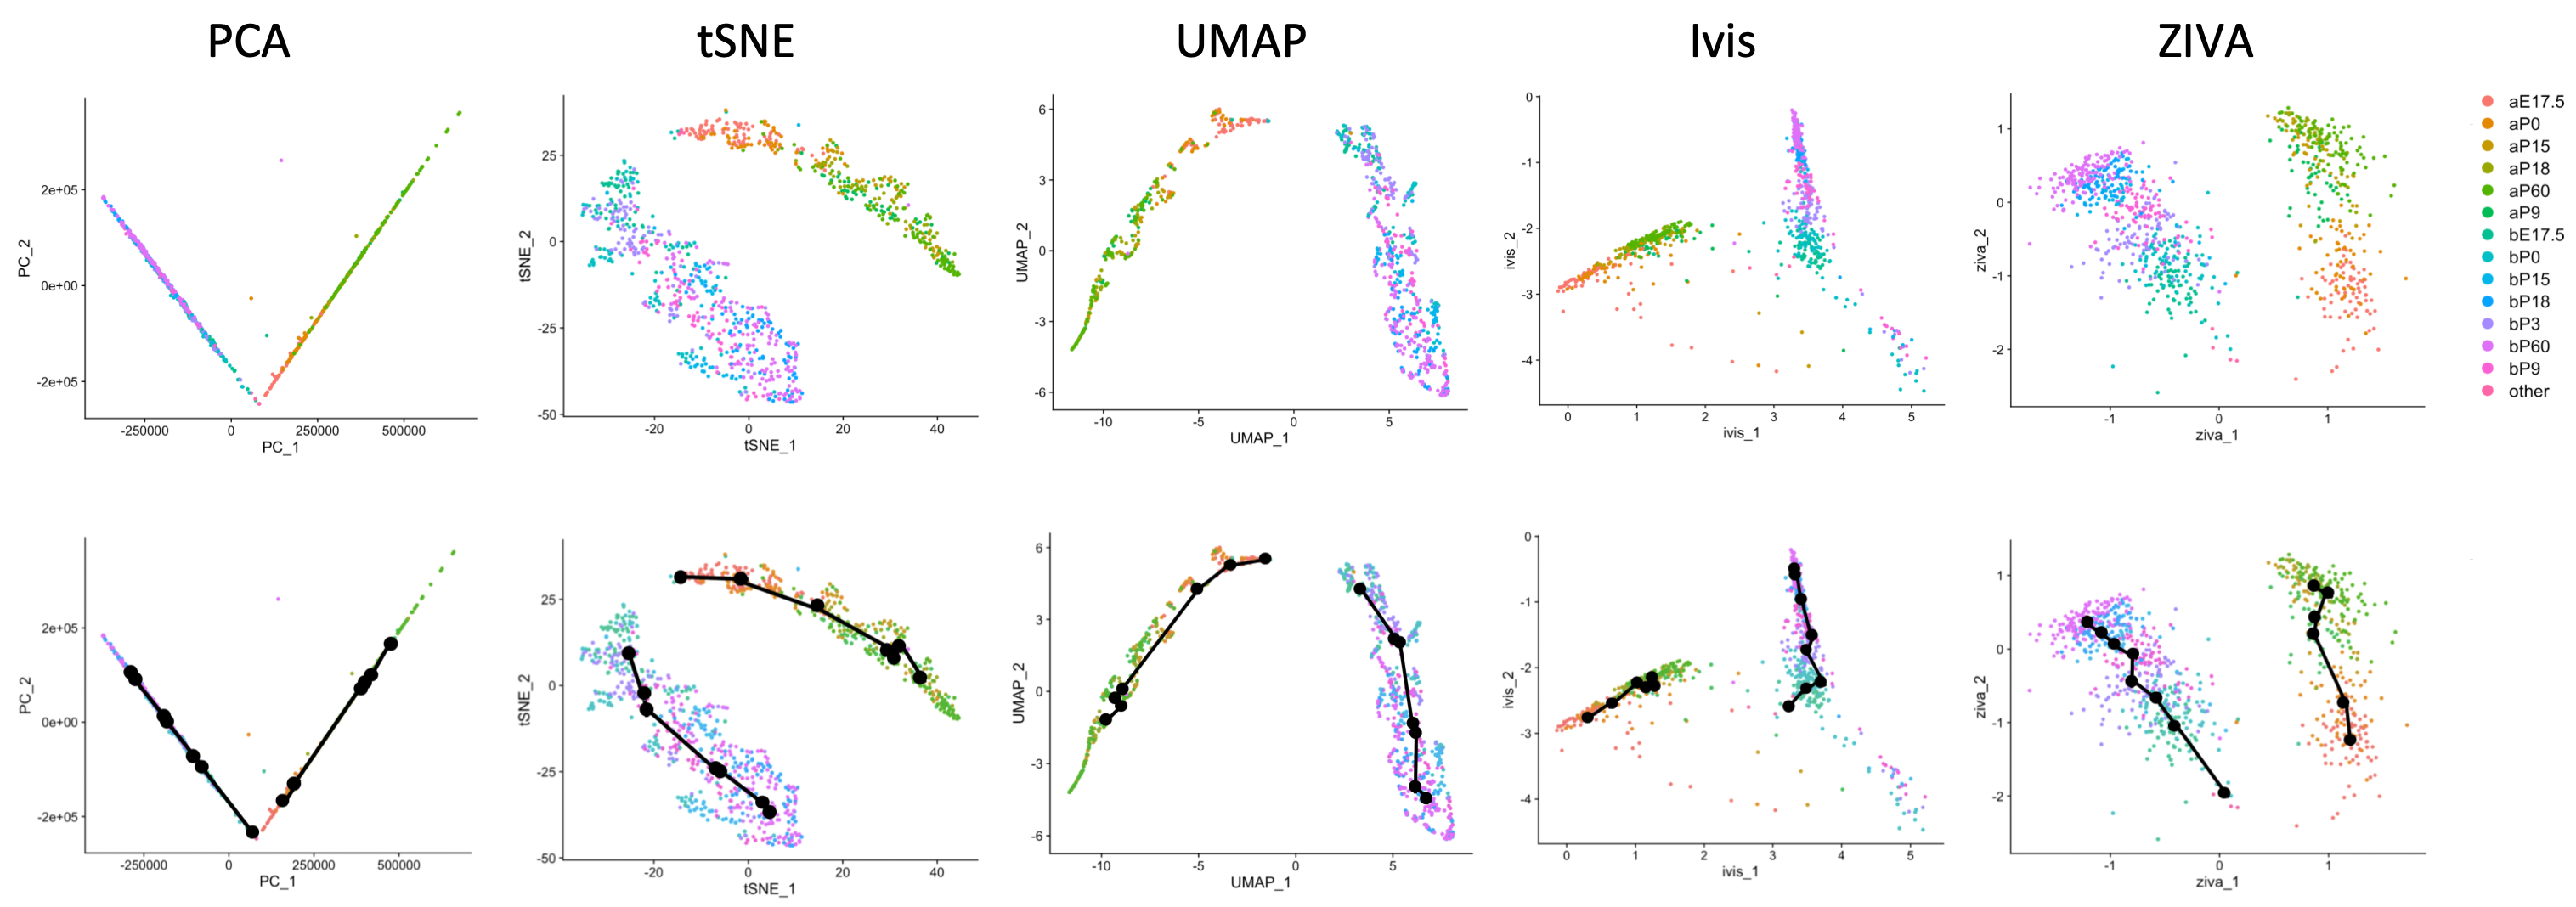
\includegraphics[width=1\textwidth]{figures/myfigures/traj.png}
    \caption{Performance of trajectory recovering of five methods}
    \label{traj}
\end{figure}


% !Mode:: "TeX:UTF-8"
% !TEX program  = xelatex
\section{\LaTeX\ 入门}
请参考 \href{https://tex.readthedocs.io/zh_CN/latest/}{在线文档},包括学习资源及学习路径。欢迎在 GitHub 上提出 \href{https://github.com/Iydon/tex/issues}{Issues}。
\clearpage

%\参考文献

 % \nocite{Nicholas1998Handbook}
  %\printbibliography[heading=none]\clearpage
  
%  % !Mode:: "TeX:UTF-8"
% !TEX program  = xelatex
\section*{数据获取函数}\label{A:data}
\Python{utils.py}{code/examples/utils.py}
\clearpage
\clearpage
% !Mode:: "TeX:UTF-8"
% !TEX program  = xelatex
\section{Supplementary materials}
\noindent\emph{Datasets} \\
To test the performance of the ZIVA method, seven datasets were used in this study. The first six datasets were downloaded from the Hemberg group (https://hemberg-lab. github.io/scRNA.seq.datasets). The seventh dataset was obtained from GEO database with accession number GSE87375.

\vspace{0.5cm}
\noindent\emph{Software and packages} \\
The PCA, tSNE and UMAP was performed using the Seurat R package from \url{https://satijalab.org/seurat/} []. It first performs normalization and scaling to the data. Then, run the three dimensionality reduction methods.\\
The ZIFA, VASC, Ivis codes was download and ran after normalization and scaling of the count data.\\
The ZIFA was performed using the package from \url{https://github.com/epierson9/ZIFA}, the block algorithm was used.\\
The codes of VASC was downloaded from \url{https://github.com/wang-research/VASC}.\\
The Ivis package was downloaded following the \url{https://github.com/beringresearch/ivis}.\\



\begin{table}[htb!]
\centering
\caption{scRNA-seq datasets used in this study}
\label{datasets}
\resizebox{13cm}{!}{
\begin{tabular}{llllllll}
\hline
No. & Dataset       & No. of cells & No. of genes & No. of types & Protocol   & Tissue       & ref \\ \hline
1   & Pollen        & 301          & 23730        & 11           & SMARTer    & Multiple     &     \\
2   & Jin           & 2610         & 2274         & 19           & inDrop     & HSPC         & Jin \\
3   & Yan           & 90           & 20214        & 6            & Tang       & Embryo Devel &     \\
4   & Camp          & 777          & 19020        & 7            & SMARTer    & Liver        &     \\
5   & Goolam        & 124          & 41480        & 5            & Smart-seq2 & Embryo devel &     \\
6   & Kolodziejczyk & 704          & 38653        & 9            & SMARTer    & Stem Cells   &     \\ \hline
\end{tabular}}
\end{table}


\begin{table}[htb!]
\centering
\caption{NMI of clustering performance of seven methods on six datasets}
\label{nmiall}
\resizebox{10cm}{!}{
\begin{tabular}{llllllll}
\hline
  & PCA  & tSNE & UMAP & ZIFA & VASC & Ivis & ZIVA \\ \hline
1 & 0.88 & 0.92 & 0.92 & 0.60 & 0.79 & 0.86 & 0.84 \\
2 & 0.57 & 0.67 & 0.71 & 0.59 & 0.65 & 0.65 & 0.67 \\
3 & 0.79 & 0.87 & 0.91 & 0.79 & 0.75 & 0.81 & 0.79 \\
4 & 0.70 & 0.78 & 0.81 & 0.60 & 0.72 & 0.81 & 0.66 \\
5 & 0.86 & 0.73 & 0.73 & 0.76 & 0.48 & 0.94 & 0.94 \\
6 & 0.70 & 0.84 & 0.87 & 0.66 & 0.25 & 0.65 & 0.60 \\ \hline
\end{tabular}}
\end{table}

\begin{table}[htb!]
\centering
\caption{NMI of clustering performance of seven methods on six datasets}
\label{ariall}
\resizebox{10cm}{!}{
\begin{tabular}{llllllll}
\hline
  & PCA  & tSNE & UMAP & ZIFA & VASC & Ivis & ZIVA \\ \hline
1 & 0.79 & 0.84 & 0.84 & 0.44 & 0.65 & 0.80 & 0.73 \\
2 & 0.34 & 0.41 & 0.48 & 0.36 & 0.39 & 0.39 & 0.43 \\
3 & 0.63 & 0.78 & 0.90 & 0.63 & 0.60 & 0.74 & 0.64 \\
4 & 0.56 & 0.61 & 0.64 & 0.42 & 0.54 & 0.70 & 0.47 \\
5 & 0.71 & 0.54 & 0.54 & 0.75 & 0.45 & 0.97 & 0.98 \\
6 & 0.48 & 0.74 & 0.77 & 0.48 & 0.11 & 0.48 & 0.43 \\ \hline
\end{tabular}}
\end{table}

\begin{table}[htb!]
\centering
\caption{NMI and ARI of clustering performance of Autoencoder, VAE and ZIVA.}
\label{t3ae}
\begin{tabular}{lllllll}
\hline
  & \multicolumn{3}{l}{NMI} & \multicolumn{3}{l}{ARI} \\ \hline
  & AE     & VAE    & ZIVA  & AE     & VAE    & ZIVA  \\ \hline
1 & 0.82   & 0.89   & 0.84  & 0.73   & 0.87   & 0.75  \\
2 & 0.64   & 0.67   & 0.67  & 0.37   & 0.41   & 0.43  \\
3 & 0.76   & 0.77   & 0.79  & 0.63   & 0.74   & 0.64  \\
4 & 0.67   & 0.69   & 0.69  & 0.48   & 0.52   & 0.51  \\
5 & 0.67   & 0.72   & 0.94  & 0.72   & 0.54   & 0.98  \\
6 & 0.58   & 0.51   & 0.60  & 0.40   & 0.33   & 0.43  \\ \hline
\end{tabular}
\end{table}

\begin{table}[htb!]
\centering
\caption{NMI and ARI of clustering performance of ZIVA under different dropout model.}
\label{tnbmm}
\begin{tabular}{lllll}
\hline
  & \multicolumn{2}{l}{NMI} & \multicolumn{2}{l}{ARI} \\ \hline
  & NB         & MM         & NB         & MM         \\ \hline
1 & 0.84       & 0.84       & 0.75       & 0.78       \\
2 & 0.67       & 0.63       & 0.41       & 0.34       \\
3 & 0.79       & 0.87       & 0.64       & 0.78       \\
4 & 0.69       & 0.68       & 0.52       & 0.51       \\
5 & 0.94       & 0.83       & 0.98       & 0.67       \\
6 & 0.61       & 0.64       & 0.44       & 0.47       \\ \hline
\end{tabular}
\end{table}


\begin{table}[htb!]
\centering
\caption{NMI and ARI of clustering performance of ZIVA under different latent dimensions.}
\label{dimt}
\begin{tabular}{lllllllll}
\hline
    & 2    & 4    & 6    & 8    & 10   & 15   & 20   & All  \\ \hline
NMI & 0.72 & 0.69 & 0.70 & 0.70 & 0.69 & 0.69 & 0.69 & 0.73 \\
ARI & 0.51 & 0.43 & 0.46 & 0.46 & 0.46 & 0.45 & 0.44 & 0.52 \\ \hline
\end{tabular}
\end{table}
%\致谢
%  % !Mode:: "TeX:UTF-8"
% !TEX program  = xelatex
\sustechthesis\ 目前版本为 \version, \LaTeX\ 毕业论文模板项目从提出到现在已有两年了。感谢为本项目贡献代码的开发人员们:
\begin{itemize}
    \item 梁钰栋(南方科技大学,本科 17 级);
    \item 张志炅(南方科技大学,本科 17 级)。
\end{itemize}
以及使用本项目,并提出诸多宝贵的修改意见的使用人员们:
\begin{itemize}
    \item 李未晏(南方科技大学,本科 15 级);
    \item 张尔聪(南方科技大学,本科 15 级)。
\end{itemize}

此外,目前的维护者并非计算机系,可能存在对协议等的错误使用,如果你在本模板中发现任何问题,请在 GitHub 中提出 \href{https://github.com/Iydon/sustechthesis/issues}{Issues},同时也非常欢迎对代码的贡献!

\end{document}
